La publicación de datos abiertos por parte de ayuntamientos e instituciones públicas está cada vez más extendido y en un futuro se irá incrementando. Estos datos son completamente accesibles y reutilizables para cualquier fin que un usuario quiera darles, lo cual da mucha libertad a la hora de crear aplicaciones y dar valor a esa información.
Esta información, en su mayoría, está publicada en formato RDF, CSV u hojas de calculo. La publicación por parte de los ayuntamientos suele contener errores, incoherencias u otros problemas que impiden su correcta utilización. Es por ello que para su uso debe hacerse un análisis y determinar una estrategia y modelización de los mismos.
\newline

En trabajo consistirá en crear una aplicación que, a partir de los datos proporcionados por el ayuntamiento de Madrid, pueda hacer una valoración de las distintas calles acorde con la seguridad de las mismas para circular en bicicleta. Todo esto siguiendo los principios de Web Semantica y Linked Data que permita realizar un buen modelado de los datos, para su correcto funcionamiento y para una posible reutilización posterior.
\newline

Primero será necesario seleccionar los vocabularios con los que se va a trabajar. Para ello se reutilizarán los ya creados en la plataforma vocab.ciudadesabiertas.es y se crearán nuevos a partir del portal de datos del ayuntamiento de Madrid (datos.madrid.es). Se reutilizará el vocabulario de Callejero, definido en \cite{ciudadesbiertas_callejero}. Y se han diseñado tres nuevos vocabularios a partir de los datasets proporcionados por el ayuntamiento de Madrid. El correspondiente a Accidentes con implicación de Bicicletas, accesible en formato CSV y XLSX en la web \cite{datosMadrid_accidentesDeBicicleta}. El correspondiente a Ciclocarriles, accesible en formato XLS y KML en la dirección 
\cite{datosMadrid_ciclocarriles}. Y el correspondiente a Calles Tranquilas, accesible en formato XLS y KML en la dirección \cite{datosMadrid_callesTranquilas}.
\newline

En este proyecto se va a desarrollar una aplicación que, a partir de estos datos y conociendo la ruta entre 2 puntos dentro de Madrid, se pueda determinar la seguridad de una ruta para ir en bicicleta. Para ello se hará uso de una API externa, de la cual se obtendrá la ruta entre las posiciones dadas por el ususario. Una vez se tengan las calles por las cuales el navegador GPS guiará al ciclista hasta su destino, se comprobará una a una su seguridad.
Para esta comprobación se hará uso de los datos mencionados antes. Para ello, se le asignará un identificador único a cada calle, el cual es proporcionado por el Callejero del ayuntamiento \cite{datosmadrid_callejero} y definido como se ha mencionado anteriormente en el portal ciudadesAbiertas. Este identificador ha sido asignado a los otros tres datasets, cuyos vocabularios han sido definidos en el contexto de este trabajo, y de esta forma es posible hacer una busqueda rápida y concisa de cada calle por la que transitará la ruta, para así conocer mejor las características de ellas y determinar su seguridad.
\newline
\newline

Más adelante se detallarán los elementos de cada vocabulario utilizado en la aplicación. En términos generales, en la siguiente figura se muestran los vocabularios definidos para este proyecto y sus enlaces con el Callejero y entre ellos.



\begin{figure}[h]
  \centering
  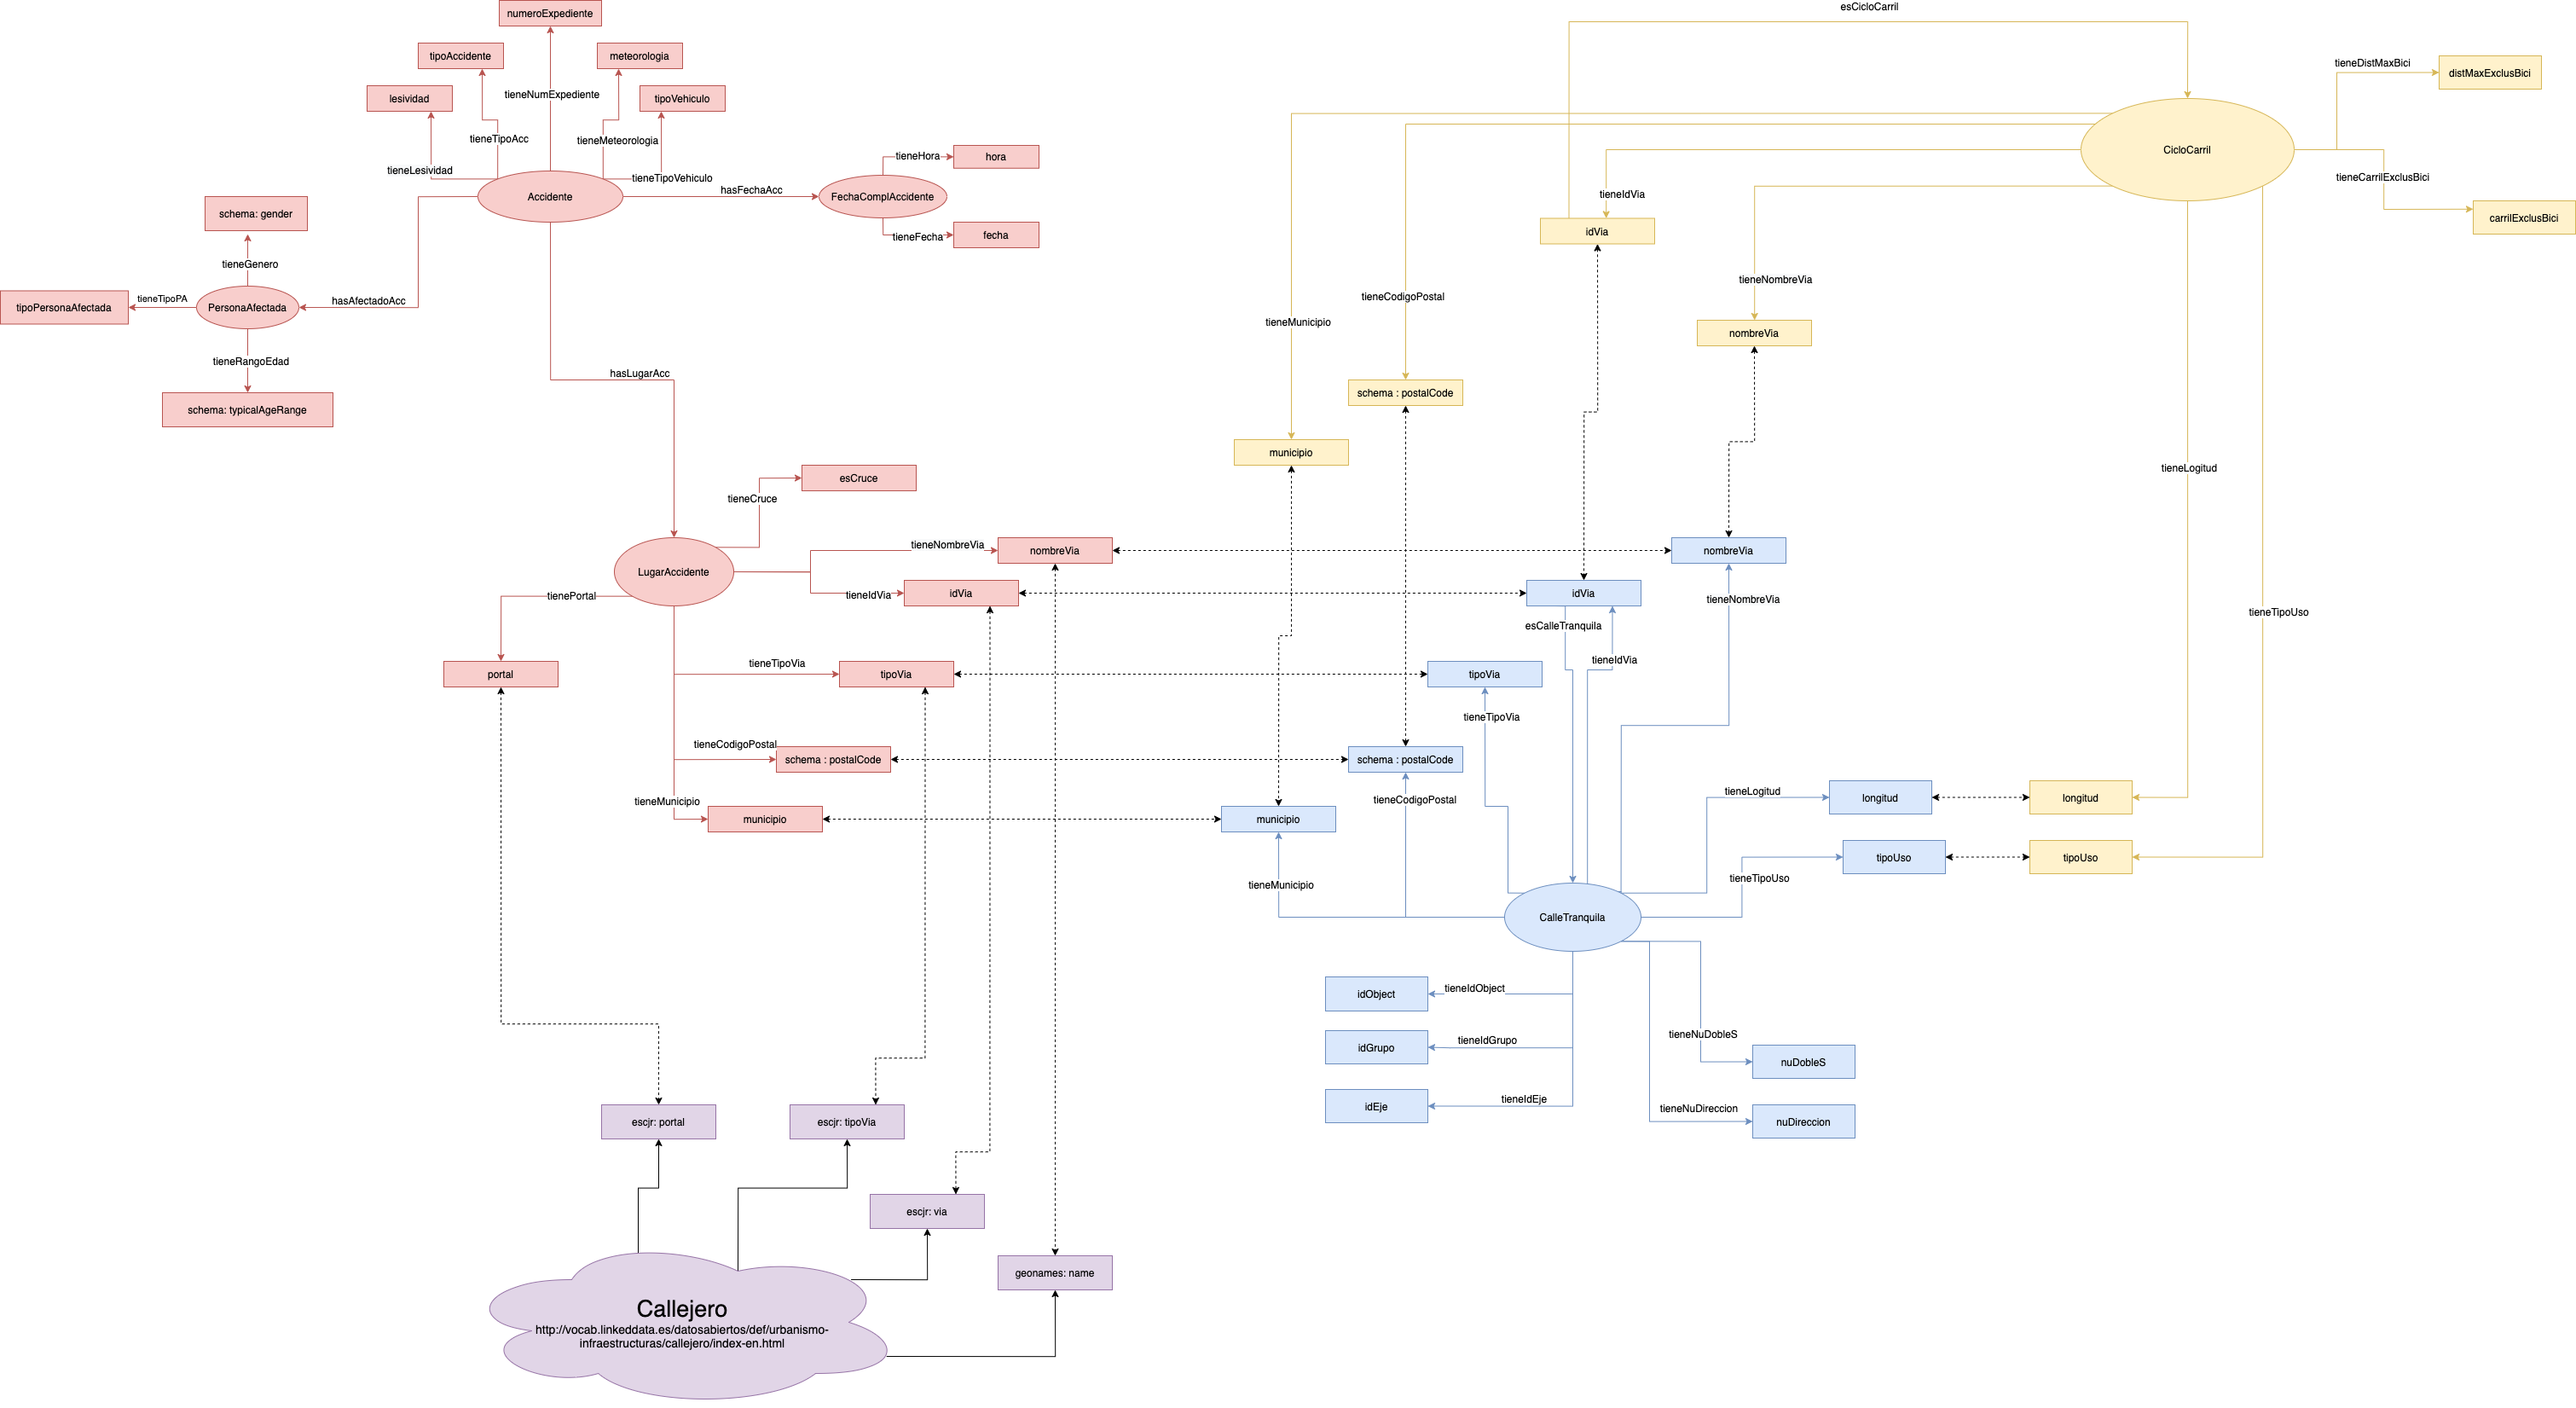
\includegraphics[angle=90, width=0.8\textwidth]{images/diagramaAppTotal.png} 
  \\
  \caption{Diagrama de los vocabularios usados en la aplicacion}
  \label{fig:esquemaTotalVocab}
\end{figure}

